\documentclass{article}
% %! Tex program = xelatex
% \documentclass{article}
%中文
%\usepackage[UTF8]{ctex}
%数学公式
\usepackage{amsmath,amssymb}
%\usepackage{ntheorem}
% \usepackage[framemethod=TikZ]{mdframed}
\usepackage{amsthm}
%边界
\usepackage[letterpaper,top=3cm,bottom=3cm,left=3cm,right=3cm,marginparwidth=1.75cm]{geometry}%table package
%Table
\usepackage{multirow,booktabs}
\usepackage{makecell}
%字体颜色
\usepackage{color}
\usepackage[dvipsnames]{xcolor}  % 更全的色系
%代码
\usepackage[OT1]{fontenc}
% MATLAB 代码风格
%\usepackage[framed,numbered,autolinebreaks,useliterate]{/Users/anye_zhenhaoyu/Desktop/Latex/mcode}
\usepackage{listings}
% \usepackage{algorithm}
\usepackage{algorithmic}
\usepackage[ruled,linesnumbered]{algorithm2e}
\usepackage{pythonhighlight} % Python
%插图
\usepackage{graphicx}
%改变item格式
\usepackage{enumerate}
%物理
\usepackage{physics}
%extra arrows
\usepackage{extarrows}
% caption(居中指令)
%\usepackage[justification=centering]{caption}
\usepackage{caption}
% htpb
\usepackage{stfloats}
% pdf 拼接
\usepackage{pdfpages}
% 超链接url
\usepackage{url}
% \usepackage{tikz}
\usepackage{pgfplots}
\pgfplotsset{compat=newest}
\usepackage[colorlinks=true, allcolors=red]{hyperref}

% --------------definations-------------- %
\def\*#1{\boldsymbol{#1}}
\def\+#1{\mathcal{#1}} 
\def\-#1{\bar{#1}}
% Domains
\def\RR{\mathbb{R}}
\def\CC{\mathbb{C}}
\def\NN{\mathbb{N}}
\def\ZZ{\mathbb{Z}}
% Newcommand
\newcommand{\inner}[2]{\langle #1,#2\rangle} 
\newcommand{\numP}{\#\mathbf{P}} 
\renewcommand{\P}{\mathbf{P}}
\newcommand{\Var}[2][]{\mathbf{Var}_{#1}\left[#2\right]}
\newcommand{\E}[2][]{\mathbf{E}_{#1}\left[#2\right]}
\renewcommand{\emptyset}{\varnothing}
\newcommand{\ol}{\overline}
\newcommand{\argmin}{\mathop{\arg\min}}
\newcommand{\argmax}{\mathop{\arg\max}}
\renewcommand{\abs}[1]{\qty|#1|}
\newcommand{\defeq}{\triangleq} % triangle over =
\def\deq{\xlongequal{def}} % 'def' over =
\def\LHS{\text{LHS}}
\def\RHS{\text{RHS}}
\def\angbr#1{\langle#1\rangle} % <x>

\def\Esolve{\textcolor{blue}{Solve: }}
\def\Eproof{\textcolor{blue}{Proof: }}
\def\case#1{\textcolor{blue}{Case \uppercase\expandafter{\romannumeral#1}: }}

% \newmdtheoremenv{lemma}{Lemma}
% \newmdtheoremenv{theorem}{\textcolor{red}{Theorem}}
% \newmdtheoremenv{defi}{\textcolor{blue}{Definition}}
\newenvironment{md}{\begin{mdframed}}{\end{mdframed}}

% \graphicspath

% \begin{document}
% \title{<++>}
\author{Charlotte Xia}
% \maketitle
% \end{document}
%! Tex program = xelatex
% \documentclass{article}
%中文
%\usepackage[UTF8]{ctex}
%数学公式
\usepackage{amsmath,amssymb}
%\usepackage{ntheorem}
% \usepackage[framemethod=TikZ]{mdframed}
\usepackage{amsthm}
%边界
\usepackage[letterpaper,top=3cm,bottom=3cm,left=3cm,right=3cm,marginparwidth=1.75cm]{geometry}%table package
%Table
\usepackage{multirow,booktabs}
\usepackage{makecell}
%字体颜色
\usepackage{color}
\usepackage[dvipsnames]{xcolor}  % 更全的色系
%代码
\usepackage[OT1]{fontenc}
% MATLAB 代码风格
%\usepackage[framed,numbered,autolinebreaks,useliterate]{/Users/anye_zhenhaoyu/Desktop/Latex/mcode}
\usepackage{listings}
% \usepackage{algorithm}
\usepackage{algorithmic}
\usepackage[ruled,linesnumbered]{algorithm2e}
\usepackage{pythonhighlight} % Python
%插图
\usepackage{graphicx}
%改变item格式
\usepackage{enumerate}
%物理
\usepackage{physics}
%extra arrows
\usepackage{extarrows}
% caption(居中指令)
%\usepackage[justification=centering]{caption}
\usepackage{caption}
% htpb
\usepackage{stfloats}
% pdf 拼接
\usepackage{pdfpages}
% 超链接url
\usepackage{url}
% \usepackage{tikz}
\usepackage{pgfplots}
\pgfplotsset{compat=newest}
\usepackage[colorlinks=true, allcolors=red]{hyperref}

% --------------definations-------------- %
\def\*#1{\boldsymbol{#1}}
\def\+#1{\mathcal{#1}} 
\def\-#1{\bar{#1}}
% Domains
\def\RR{\mathbb{R}}
\def\CC{\mathbb{C}}
\def\NN{\mathbb{N}}
\def\ZZ{\mathbb{Z}}
% Newcommand
\newcommand{\inner}[2]{\langle #1,#2\rangle} 
\newcommand{\numP}{\#\mathbf{P}} 
\renewcommand{\P}{\mathbf{P}}
\newcommand{\Var}[2][]{\mathbf{Var}_{#1}\left[#2\right]}
\newcommand{\E}[2][]{\mathbf{E}_{#1}\left[#2\right]}
\renewcommand{\emptyset}{\varnothing}
\newcommand{\ol}{\overline}
\newcommand{\argmin}{\mathop{\arg\min}}
\newcommand{\argmax}{\mathop{\arg\max}}
\renewcommand{\abs}[1]{\qty|#1|}
\newcommand{\defeq}{\triangleq} % triangle over =
\def\deq{\xlongequal{def}} % 'def' over =
\def\LHS{\text{LHS}}
\def\RHS{\text{RHS}}
\def\angbr#1{\langle#1\rangle} % <x>

\def\Esolve{\textcolor{blue}{Solve: }}
\def\Eproof{\textcolor{blue}{Proof: }}
\def\case#1{\textcolor{blue}{Case \uppercase\expandafter{\romannumeral#1}: }}

% \newmdtheoremenv{lemma}{Lemma}
% \newmdtheoremenv{theorem}{\textcolor{red}{Theorem}}
% \newmdtheoremenv{defi}{\textcolor{blue}{Definition}}
\newenvironment{md}{\begin{mdframed}}{\end{mdframed}}

% \graphicspath

% \begin{document}
% \title{<++>}
\author{Charlotte Xia}
% \maketitle
% \end{document}
\usepackage{fancyhdr}
\pagestyle{fancy}
\fancyhead[L]{\slshape{Charlotte Xia}}

% theorems
\usepackage{thmtools}
\usepackage{thm-restate}
\usepackage[framemethod=TikZ]{mdframed}
\mdfsetup{skipabove=1em,skipbelow=0em, innertopmargin=12pt, innerbottommargin=8pt}

\theoremstyle{definition}

\declaretheoremstyle[headfont=\bfseries\sffamily, bodyfont=\normalfont,
	mdframed={
		nobreak,
		backgroundcolor=brown!14,
		topline=false,
		rightline=false,
		leftline=true,
		bottomline=false,
		linewidth=2pt,
		linecolor=brown!180,
	}
]{thmbrownbox}

\declaretheoremstyle[headfont=\bfseries\sffamily, bodyfont=\normalfont,
	mdframed={
		nobreak,
		backgroundcolor=Blue!4,
		topline=false,
		rightline=false,
		leftline=true,
		bottomline=false,
		linewidth=2pt,
		linecolor=NavyBlue!120,
	}
]{thmbluebox}

\declaretheoremstyle[headfont=\bfseries\sffamily, bodyfont=\normalfont,
	mdframed={
		nobreak,
		backgroundcolor=Green!5,
		topline=false,
		rightline=false,
		leftline=true,
		bottomline=false,
		linewidth=2pt,
		linecolor=OliveGreen!120,
	}
]{thmgreenbox}

\declaretheoremstyle[headfont=\bfseries\sffamily, bodyfont=\normalfont,
	mdframed={
		nobreak,
		topline=false,
		rightline=false,
		leftline=true,
		bottomline=false,
		linewidth=2pt,
		linecolor=OliveGreen!120,
	}
]{thmgreenline}

\declaretheoremstyle[headfont=\bfseries\sffamily, bodyfont=\normalfont,
	mdframed={
		nobreak,
		topline=false,
		rightline=false,
		leftline=true,
		bottomline=false,
		linewidth=2pt,
		linecolor=NavyBlue!70,
	}
]{thmblueline}

\declaretheorem[numberwithin=section, style=thmbrownbox, name={\color{Brown}Definition}]{defi}
\declaretheorem[numberwithin=section, style=thmgreenbox, name={\color{OliveGreen}Law}]{law}
\declaretheorem[numberwithin=section, style=thmbluebox, name={\color{Blue}Corollary}]{cor}
% 可以由Theorem直接推出来的东西
\declaretheorem[numberwithin=section, style=thmgreenline, name={\color{OliveGreen}Property}]{prt} 
\declaretheorem[numberwithin=section, style=thmbluebox, name={\color{Blue}Proposition}]{prp} 
% 一个比较特例的内容,它可能只对我们这篇文章里面的东西有用,也许是某个一般性性质的特殊应用,也许是专门要计算这么一部分内容,总之不一定适合给别人引用,没有稍微宽一点的普适性(但是Lemma可以有)。感觉是比较综合Lemma,Corollary和Remark的性质。
\declaretheorem[numberwithin=section, style=thmbluebox, name={\color{Blue}Theorem}]{thm} 
% 全文中最重要的(几个)内容,我写这篇文章就是要告诉读者这件事。也可以是某一章最重要的内容,说这一章我们就干这件事了,放在全文可能是main Theorem的一步。
\declaretheorem[numberwithin=section, style=thmbluebox, name={\color{Blue}Lemma}]{lemma}
% 和Theorem比没有那么重要,但是对于我们现在关注的Theorem有直接的作用,比如是拆解Theorem成几个不同的方向,后面要合起来,方便读者理解。
\declaretheorem[numberwithin=section, style=thmbrownbox,  name={\color{NavyBrown}Example}]{eg}
\declaretheorem[numberwithin=section, style=thmgreenline, name={\color{OliveGreen}Remark}]{remark}
\declaretheorem[numbered=no,style=thmblueline, name={\color{NavyBlue!70}Proof},qed=$\square$]{prf}

\begin{document}
\title{mid-term cheatsheet}
\maketitle
\section{Divide and Conquer}
\subsection{Master Theorem}
If $T(n)=aT(\frac{n}{b})+O(n^d)$, where a: num of subproblems; b:subproblem size n/b; d: combining time complexity.\\
$O(n^d)$:combining time complexity\\
\begin{equation}
    T(n)=
    \begin{cases}
        O(n^d) & \text{if } a<b^d\\
        O(n^{\log_b a}) & \text{if } a>b^d \\
        O(n^d \log n) & \text{if } a=b^d\\
    \end{cases}    
\end{equation}

\subsection{Karatsuba algorithm}
For bottom layer, $3^{\log_2n}=n^{\log_23}=n^{1.6}$ subproblems with linear opertion time. $T(n)=3T(\frac{n}{2})+O(n)$.
\begin{algorithm}
    \caption{Karatsuba algorithm}
    \textbf{Input:}Two n-digit numbers $x,y$. \\
    \textbf{Output:} their product\\
    $x_L,x_R=\text{leftmost} \lceil n/2\rceil ,\text{rightmost} \lfloor n/2 \rfloor $ bits of x\\
    $y_L,y_R=\text{leftmost} \lceil n/2\rceil ,\text{rightmost} \lfloor n/2 \rfloor $ bits of y\\
    P1=multiply($x_L,y_L$) \\
    P2=multiply($x_R,y_R$) \\
    P3=multiply($x_L+x_R,y_L+y_R$) \\
    return $P1\times 2^n+(P3-P1-P2)\times 2^{\frac{n}{2}}+P2$
\end{algorithm}

\subsection{Inversions}
\begin{algorithm}
    \KwIn{S=($x_1, x_2, \ldots , x_{n}$),A:$x_1, x_2, \ldots , x_{n/2}$; 
    B:$x_{n/2+1}, x_{n/2+2}, … , x_n$}
    \KwOut{Number of Inversions: count}
    count=0\\
    \If{$n==1$}{
        \Return{0}\\
    }
    count+=countInversions(A)+countInversions(B)\\
    Maintain 2 pointers $i=1,j=n/2+1$; C=\{\}\\
    \While{$i < n/2$ and $j < n$}{
        \If{$x_i<x_j$}{
            C.append($x_{i++}$)\\
        }
        \Else{
            C.append($x_{j++}$)\\
            $count+=j-n/2$
        }
    }
    count+=(n/2-i)$\times $(j-n/2) \# B reached end, while remaining numbers in A are bigger than all B\\
    S=C\\
    \Return{count}
    \caption{countInversions}
\end{algorithm}

\subsection{Selection}
For \textbf{selection}, worst $O(n)$, best $O(\log n)$. For \textbf{quick sort}, if pivot chosen by median of medians, $O(n\log n)$, worst $O(n^2)$.
\begin{algorithm}
    \caption{Select}
    Choose an \textbf{arbitrary} value $v$ among $x_1,x_2,\ldots,$\\
    Divide $x_1,x_2,\ldots,x_n$ into three subsets $L,M,R$\\
    \If{$k\leq |L|$}{
        return Select(L,k)
    }
    \ElseIf{$|L| < k \leq  |L|+|M|$}{
        return $v$
    }
    \ElseIf{$|L|+|M| < k$}{
        return Select(R,$k-|L|-|M|$)
    }
\end{algorithm}

\subsection{median of medians}
$T(n)=T(n/5)+T(7n/10)+O(n)$\\
Assume that $T(n) \leq cn$,
$T(\frac{n}{5})<\frac{cn}{5}$,$T(\frac{7n}{10})<\frac{7cn}{10}$,
$T(n)=T(\frac{n}{5})+T(\frac{7n}{10})+O(n)<0.9cn+bn\leq cn$. which holds when we set c to be bigger then b.

\subsection{Closest Pair}
If we sort by y-cordinate every merge step, $O(n\log n^2)$, can be improved to $O(n\log n )$ by pluging it into merge opertation.
\begin{algorithm}
    \caption{FindClosestPair}
    \KwIn{A list of pairs P: $p_1=(a_1,b_1),\ldots p_i=(a_i,b_i),\ldots,p_n=(a_n,b_n)$}
    \KwOut{distance of closest two pairs in P: dist}
    Sort P by x-coordinate. \# $O(n\log n)$\\
    Divide P into two equally sized subsets A,B, the point in the middle $p_{mid}=(a_{mid},b_{mid})$.\\
    dist=min(\textbf{FindClosestPair(A)},\textbf{FindClosestPair(B)})\\
    Merge A and B by y-cordinate to form C.\\
    \ForEach{$c_i=(a_i,b_i) $ in C}{
        \If{$|a_i-a_{mid}|<dist$}{ add $c_i$ to S}
    }

    \ForEach{$s_i=(a_i,b_i) $ in S}{
        j=i+1\\
        \While{$| b_i - b_{j}| <dist$}{
            dist=min(dist, $\| b_i - b_{i+1}\|$)\\
            j=j+1\\
        }
    }
    \Return{dist}
\end{algorithm}
\section{Graph}
\subsection{DFS}
\begin{enumerate}
    \item \textbf{Tree Edges} Edges in the DFS search: (u, v) where marked(v) = false
    \item \textbf{Forward Edges} Edges that point to non-child descendants
    \item \textbf{Back Edges} Edges that point to ancestors
    \item \textbf{Cross Edges} All the other edges: edges point to vertices on other tree
    doesn't exist for undirected graph, since if $(c,f)$ occurs it will only be tree edge.
\end{enumerate}

\begin{figure}[htbp]
	\centering
	\begin{minipage}{0.5\linewidth}
		\centering
		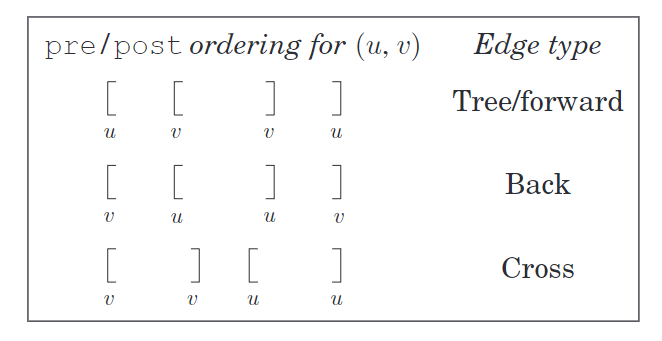
\includegraphics[width=0.8\linewidth]{fig/edgeType.png}
		\caption{Directed Graph}
        \label{fig:edgeGraph}
    	\end{minipage}
	%\qquad
	\begin{minipage}{0.4\linewidth}
		\centering
		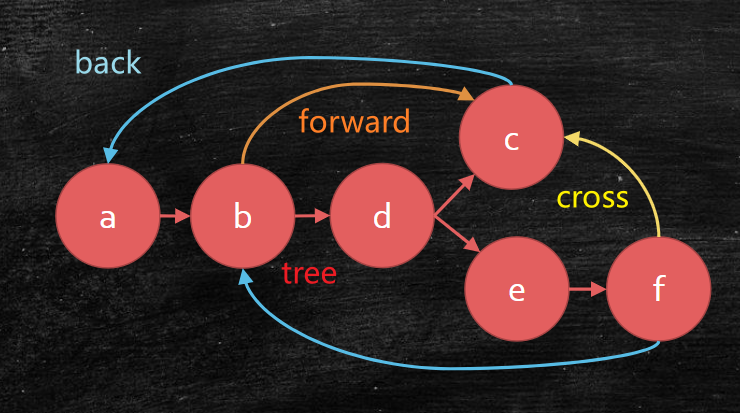
\includegraphics[width=0.8\linewidth]{fig/edgeTypeFigure.png}
		\caption{colored edges}
		\label{fig:colored}%文中引用该图片代号
	\end{minipage}
\end{figure}
\begin{algorithm}
    \caption{DFS on Directed Graph}
    \label{alg:dfs}
    \SetKwFunction{explore}{explore}
    clk=0\\
    \ForEach{$v \in V$}{
        \If{marked[v]=False}{
            \explore{$v$} \\
            clk++ \# used to calculate the number of connected components\\
        }
    }
    \SetKwFunction{explore}{explore}
    \SetKwProg{Fn}{Function}{:}{}
    \Fn{\explore{$u$}}{
        pre[u]=clk\\
        clk++\\
        visited[u]=false\\
        \ForEach{$(u,v) \in E$}{
            \If{marked[v]=false}{
                \explore($v$)
            }
        }
        post[u]=clk\\
        clk++\\
    }
\end{algorithm}
\subsection{strongly connected components}  
\begin{itemize}
    \item Note that we can't simply employ DFS to find C.C., as although you find reachable points from a certain vertice $v$, the vertice you explore may not be reachable from each other.
    \item Note that unlike topological ordering, the node with the earliest post time doesn't necessarily occur in sink SCC,
    as the vertice with outer edges are previsited where our algorithm ends in somewhere else.i.e.,for graph \ref{fig:SCC} consider DFS in sequence {5,6,7,8}, apparently, the 8 has the smallest post value, but is not in sink.
    \item However, the vertice with biggest post time must be in source SCC. 
    Assume $u$ has the largest finish time, which must be a root of one DFS tree. Suppose $u$ isn't in source SCC, i.e. $\exists v$ s.t. $(v,u)$ exists. 
    $v$ isn't in the tree of $u$, as $(u,v)$ doesn't exist.
    ,$v$ cannot start earlier than $u$, $v$ isn't in another DFS tree. 
    \item Consider the meta-graph, where connected components form a big node, it must be DAG, else contradict with biggest SCC, therefore, there must be a sink. Also, a way to find whether $v$ is reachable from $u$ is to check the connectivity of bigger SCCs, $U$ and $V$. 
    
\end{itemize}

\begin{algorithm}
    \caption{Strongly Connected Component}
    \label{alg:SCC}
    \KwIn{DAG:G}
    \KwOut{num of SCC}
    Deduce G's inverse $G^R$ from G\\
    Run DFS on $G^R$ to find source SSC, which is sink SSC of $G$, record it in the descending finish time as F.\\
    DFS on $G$ in the order of F.
\end{algorithm}
\subsection{BFS}
\begin{algorithm}
    \caption{alg:bfs}
    \label{Naive BFS}
    \SetKwFunction{bfs}{bfs}
    Queue Q;\\
    \SetKwProg{Fn}{Function}{:}{}
    \Fn{\bfs{,$Q$,$u$}}{
        \textbf{for each} $v \in V$ $marked[v] \leftarrow false$\\
        Q.push(s)
        $marked[s]\leftarrow true$
        \While{Q is not empty}{
            u=Q.top();Q.pop();\\
            \ForEach{$(u,v) \in E$}{
                \If{marked[v]=false}{
                    marked[v]=True\\
                    Q.push(v)
                }
            } 
        } 
    }
\end{algorithm}
\subsection{Dijkstra}
Dijkstra's algorithm runs on positive-edge graph. It updates all vertice connected to the visited set and drag the closest vertex into the set. We conduct $|V|$ insert and $|E|$ update, each operation taking $O(\log n)$, $O((|E|+|V|)\log|V|)$. 
If there exists $x \notin SPT, v \in SPT$, s.t. $dist(s\rightarrow x \rightarrow v)<dist(v)$, $dist(x)<dist(v)$, $x$ should be in $SPT$,contradiction! 
\begin{algorithm}
\caption{Di(j)kstra}
\label{fig:dijk}
\KwIn{G=(V,E),s}
\KwOut{dist(u) is the shortest distance from s to u}

\ForEach{$u \in V$}{
    dist(u)=$\inf$\\
    pre(u)=Nan \# initialize
}
dist(s)=0\\
H=makequeue(V)\\
\While{H is not empty}{
    u=H.top();H.pop()\\
    \ForEach{$(u,v) \in E$}{
        \If{$dist(v)>dist(u)+l(u,v)$}{
            $dist(v)=dist(u)+l(u,v)$ \# update the shortest dist \\
            pre(v)=u\# record previous node\\
        }
    }
}
\end{algorithm}

\subsection{Bellman-Ford}
The key idea of Bellman-Ford is that it updates all the edges (kind of 'edgewise' operation) each time (different from Dijkstra's algorithm who updates nodes one step connected to SPT), which takes $O(|V||E|)$.

\begin{algorithm}
    \KwIn{G=(V,E),s}
    \caption{Bellman-Ford}
    dist[s]=0, dist[x]=$\inf$ for vertex other than s\\
    pre(v)=Nan\\
    \While{some dist[x] updates}{ \# update at most $|V|$ rounds.
        \ForEach{$(u,v) \in E$}{
            \If{$dist[v]>dist[u]+w(u,v)$}{
                dist[v]=dist[u]+w(u,v)\\
                pre(v)=u\\
            }
        }
    }
\end{algorithm}
\textbf{Correctness of algorithm:}
\begin{enumerate}
    \item After k rounds, dist(v) is the shortest path of all k-edge-paths.($dist[u_k]\leq d(u_1,u_2,\ldots,u_k)$)\\
    For base step, dist[s] is the shortest dist of all 0-edge-paths.\\
    For induction step, suppose it is true for $k-1$ rounds, $dist[u_{k-1}] \leq d(u_1,\ldots,u_{k-1})$. By Bellman-ford update condition, $dist[u_{k}]\leq d(u_1,\ldots,u_{k-1})+w(u_{k-1},v)$, the righthand side means all the other k-edge-paths.
    \item For graphs without negative cycle, all the shortest paths will have at most $|V|-1$ edges.
    
    If there are more than $|V|$ paths, a vertex must be visited twice, but by erasing the whole cycle results in a shorter path, contradiction!
    \item Negative cycle exists iff some dist is updated in the last($|V|^{th}$) round.
    \item If no vertice updates in $V^{th}$ round, then no vertice will be updated then. But if a single vertice is not updated.
    \item If a vertex is upgraded after $V$ rounds, then its path must include a negative cycle.
    A negative cycle can be found by tracing the recorded shortest path until two repeated nodes occurs. Tricks include running till the $2|V|^{th}$ round and see the vertice upgraded in $|V|^{th}$ and $2|V|^{th}$.
\end{enumerate}

\section{Greedy Algorithm}
\subsection{Prim}
Adding the edge out of the previous Tree $T_i$ with the minimum weight to form $T_{i+1}$.\\
\textbf{Correctness of algorithm:}

The key idea for Prim is to guarantee that the tree with $n$ edges $T_n$ is a subset of \textbf{global} MST $T$. 
In inductive step, if $T_{i}$ is part of $T$, then we can construct $T_{i+1}$, s.t. $T_{i+1}\in T$.
Consider the first edge $e$ out of $T_{i}$, if $e=(u,v) \notin T$, then adding $e$ to $T$ constructs a cycle $C$. 
Since $e$ rather than $e' \in C, e' \notin T_{i}, e' \in T$, $w(e')\geq w(e)$. Since $T$ is the smallest spanning tree, $T-w(e')+w(e)\geq T$, $w(e)\geq w(e')$, therefore, $w(e)=w(e')$. Therefore, by shifting the two edges guarantees $T_{i+1}$ is a MST component of $T$.\\
\textbf{Time complexity:} $O((|E|+|V|)\log(|V|))$.\\
\subsection{Kruskal}
$O(|E|\log(|E|))$ for sorting edges, and $|E|$ iterations of finding the representative element. A faster data structure is by \textbf{unified set}, which is $O(|E|\log(|V|))$ \\
\begin{algorithm}
    \caption{Kruskal's Algorithm}
    \SetKwFunction{union}{union}
    \SetKwFunction{mk}{makeset}
    \SetKwFunction{find}{find}
    \SetKwProg{Fn}{Function}{:}{}

    Sort the edge set E to ascending order.\\
    X=\{\}\\
    For each $u\in V$, makeset($u$).  \# $|V|$ create group\\
    For each $(u,v) \in E$ in ascending order\\
    \If {$find(u) \neq find(v)$}{
        Add edge $(u,v)$ to X\\
        \union(u,v)\\
    }
    \Fn{\mk{$x$}}{
        $\pi(x)=x$\\
        $rank(x)=0$
    }
    \Fn{\find{$x$}}{
        \While{$\pi(x) \neq x$}{
            $\pi(x)$=\find($\pi(x)$)
        }
        \Return{$x$} \# path Compression
    }
    \Fn{\union{$x$,$y$}}{
        $r_x=find(x)$ \# $r_x$ means root(representative) of x\\
        $r_y=find(y)$\\
        \If{$r_x=r_y$}{
            \Return{} \# already in the same group
        }
        \If{$rank(r_x)>rank(r_y)$}{
            $\pi(r_y)=r_x$ \# merge the smaller tree to the bigger tree
        }
        \If{$rank(r_x)=rank(r_y)$}{
            $rank(r_y)=rank(r_y)+1$
            }
        }
\end{algorithm}
\subsection{set coverage}
    Denote $S_l=\{A_1,\ldots A_l\}$ as the out put of greedy after $l$ iterations, $S^*=\{O_1,\ldots, O_k\}$ be \textbf{any} collection of $k$ subsets.
\[f(S_l)\geq (1-(1-1/k)^l)f(S^*)\]
% where $f(S^*)$ is the optim. sol. 
    For base step, $l=1$,by greedy nature, $f(S1={A1})\geq f({O_i})$ for all $O_i$.
    Thus $f(S_1)\geq \frac{1}{k}\sum_{O_i \in S^*}f({O_i})=(1-(1-\frac{1}{k})^1)f(S^*)$ This implies when calculating the sum, union elements are calculated more than once.
    Also, the size of the first chosen set is larger than the average size of the optimal solution.
    Denote $\Delta(O_i|S_t)=f(S_t\cup {O_i})-f(S_t)$.
    $\Delta(A_{t+1}|S_t)\geq\frac{1}{k}\sum_{i=1}^k\Delta(O_i|S_t) \geq \frac{1}{k}\Delta(S^*|S_t)$.\\
    For inductive step, suppose $f(S_t)\geq (1-(1-1/k)^t)f(S^*) $ 

    $f(S_{t+1})-f(S_t)\geq \frac{1}{k}(f(S^*\cup S_t)-f(S_t))\geq \frac{1}{k}(f(S^*)-f(S_t))$.
    
    $f(S_{t+1})\geq \frac{1}{k}f(S^*) + (1-\frac{1}{k})f(S_t)
    \geq \frac{1}{k}f(S^*) + (1-\frac{1}{k})(1-(1-1/k)^t)f(S^*)=((1-(1-1/k)^{t+1})f(S^*))$.\\
For max-k-coverage, we at most choose $k$ sets.
$\lim_{k\rightarrow \infty}(1-(1-1/k)^l) =1-1/e$.\\
For set cover problem, it is a $ln n$ approximation. Suppose $|S^*|=k$ is optimal(f($S^*$)=n).
$f(S)\geq (1-(1-1/k)^{k\cdot ln n})f(S^*)>(1-1/e^{ln n})f(S^*)=n-1$ Therefore, $f(S)=n$.

\subsection{Huffman Coding}
The more frequent an encoding appears, the shorter the encoding is.
    Denote $T$ as the Huffman Tree, and $T'$ the tree that switched $u,v$, where $len(u)<len(v)$, $w(u)>w(v)$.
    avg\_len(T)-avg\_len(T')=$w(u)\cdot len(u)+w(v)\cdot len(v)-w(v)len(u)-w(u)len(v)=(w(u)-w(v))(len(u)-len(v)) <0$.

    Next, we'll guarantee that every next step is optim, i.e. $T_{i-1}$ is part of $T$.
    For base step,...
    For inductive step: If we merge $A$ and $B$ in $T$. If $A$ is paired with $C$ in $T^*$, then $w(C)>w(A)$ ,$w(B)\leq w(C)$. If $w(B)=w(C)$, changing B and C preserves avg\_len.
    If $w(B) < w(C)$, $len(B)\geq len(C)$ by above proof. If $len(B)==len(C)$, swapping B and C also preserves avg\_len. If $len(B)>len(C)$, D is not processed, $w(D)> max(w(A),w(B))$, but $len(D)=len(B)>len(C)$, contradict with the fact that $T^*$ is optimal(by above proof).

    Another intepretation is by sorting inequality, namely, the sum of $\sum ordered\_sequence \leq \sum random\_sequence \leq \sum inversed\_sequence$.

    \textbf{time complexity:} By using binary-heap, every time we conduct pop twice to obtain the top two min vertice and a push to add the new parent vertice in the tree, which takes $O(n\log n)$.

    \subsection{k-center}
    \begin{itemize}
    \item \textbf{Algorithm:} Iteratively pick the center farthest to the existing centers. Pick the first by random. by Dijkstra for weighted graph and BFS for unweighted.\\
\item The algorithm is \textbf{2-approximation}.

Denote $OPT=\max \min d(o_1,v)$. $A=\{a_1,\ldots a_k\}$ for algorithm result, $X_i=\{v_1,\ldots v_i\}$ as the set of vertice closest to $o_i$, optim solution $O=\{o_1,\ldots, o_k\}$

Case 1:Suppose $A\cap X_i \neq \emptyset$ for all $i$. Then each $X_i$ contains a center, as the biggest length between two vertice in $X_i$ is smaller than $2OPT$ by triangle inequality.

Case 2:Suppose $\exists A \cap X_i =\emptyset$. Suppose we choose $a_j$ and $a_r\in X_i$. Let $a_r$ be the second center chosen in $X_i$.
By greedy choice, before $a_r$ was chosen, the algorithm answer $ALG =d(A,a_r)\leq d(a_j,a_r)$ . Additionally, $d(a_j,a_r)\leq d(a_j,o_i)+d(a_r,o_i)\leq 2OPT$.
    \end{itemize}
\subsection{max-cut}
\begin{itemize}
    \item  Start with any partition $\{A,B\}$.
If moving a vertex $u$ from $A$ to $B$ or from $B$ to $A$ increases 
$c(A,B)$, move it. Terminate until no such movement is possible
    \item \textbf{Time Complexity} checking whether to update takes $O(|E|)$, every update you earns at least an edge, so it takes $O(|E|)$ rounds. The total algorithm is $O(|E|^2)$, polynomial!
    \item \textbf{Approximation} When the algorithm terminates, $\forall u$, at least 0.5deg(u) edges are in the cut, which leads to a 0.5-approximation.
     \[c(A,B)\geq \frac{1}{2}\sum_{u\in V}\frac{1}{2}deg(u)=\frac{1}{2}|E|\]
\end{itemize}

\end{document}